%Compile with PDFLaTeX
\documentclass[a4paper,10pt,english]{article}
\usepackage{mathptmx}
\renewcommand{\familydefault}{\rmdefault}
\usepackage{graphicx}
\usepackage{babel}
\usepackage{caption}
\usepackage{subcaption}
\usepackage{floatrow}
\usepackage{orstylet}
\makeatother
\begin{document}
\renewcommand{\figurename}{Fig.} 


\title{FAKE LEPTON BACKGROUND STUDY FOR DRELL-YAN DIFFERENTIAL CROSS SECTION MEASUREMENT}


\author{\uline{Marijus Ambrozas}, Andrius Juodagalvis}

\maketitle

\address{Institute of Theoretical Physics and Astronomy, Faculty of Physics, Vilnius University, Lithuania}

\rightaddress{marijus.ambrozas@ff.stud.vu.lt}

The Large Hadron Collider (LHC) at CERN accelerates protons to almost the speed of light and collides them together
with $13$ TeV collision energy.
Short-lived heavy particles may be produced during such collisions, and investigation of these events allows physicists
to further push the frontier of our understanging about the Universe.
Colliding protons can be described as two opposite flows of quarks and gluons, according to the parton model.
Any two (or more) partons may interact during the collision, producing new particles.
There are different probabilities of different outcomes, which depend on parton distribution functions (PDFs).
PDFs describe probabilities of existance of specific partons inside a proton.
PDFs must be measured with high precision in order to make correct predictions about particle interactions.

The Drell-Yan process takes place during a proton-proton collision, when a quark and an antiquark annihilate to create
a $Z$ boson or a virtual photon which nearly instantly decays into a lepton-antilepton pair (dilepton for short) \cite{DY}.
Dilepton center-of-mass properties depend directly on four-momenta of the annihilating quarks.
Therefore, precise measurements of Drell-Yan process differential cross sections are used for constraining the PDFs \cite{DY13}.
These measurements are also useful for testing the validity of higher-order corrections of the standard model as
well as for a number of other experimental measurements where the Drell-Yan process is considered a bacground \cite{Higgs, Zprime, SUSY}.

Leptons created during the Drell-Yan process usually have a high momentum and leave tracks that are well separated
from tracks of other particles.
This type of leptons is usually called ``prompt''.
There also are other processes that may produce prompt lepton pairs just like the Drell-Yan process.
We refer to these processes as prompt lepton backgrounds.
There is also, however, a possibility that a poorly isolated lepton emerging from a hadronic jet or even the jet itself
will be misreconstructed as a prompt lepton.
This type of leptons is called `fake'.
Typical fake lepton backgrounds are $W\!+\!\mathrm{Jets}$ (one lepton is prompt and one is fake) and $QC\!D$ multijet
(both leptons are fake).

Fake lepton events have very large cross sections and very low probabilities to be selected as Drell-Yan event candidates.
Therefore, simulated fake lepton background predictions are usually very inaccurate.
Data-driven techniques are exploited to estimate such background yields.
The ``fake rate'' method relies on measuring fake lepton selection efficiency (sometimes called in jargon as ``fake rate'').
Measured efficiency is used with events containing fake leptons that have failed the selection to estimate the number of
events that have passed it.
In theory, a more sophisticated method is the so called ``matrix method'', which, in addition to fake lepton efficiency,
includes the measurement of prompt lepton selection efficiency.
Both methods will be presented and compared in the context of Drell-Yan differential cross section measurement using
2016 CERN CMS data.

The work was financed by Vilnius University Experimental Nuclear and Particle Physics Center and done in collaboration with
scientists from Universit\'{e} libre de Bruxelles, Seoul National University, and University of Nebraska Lincoln.
 
\vspace{-0.3cm}
\begin{figure}[H]
	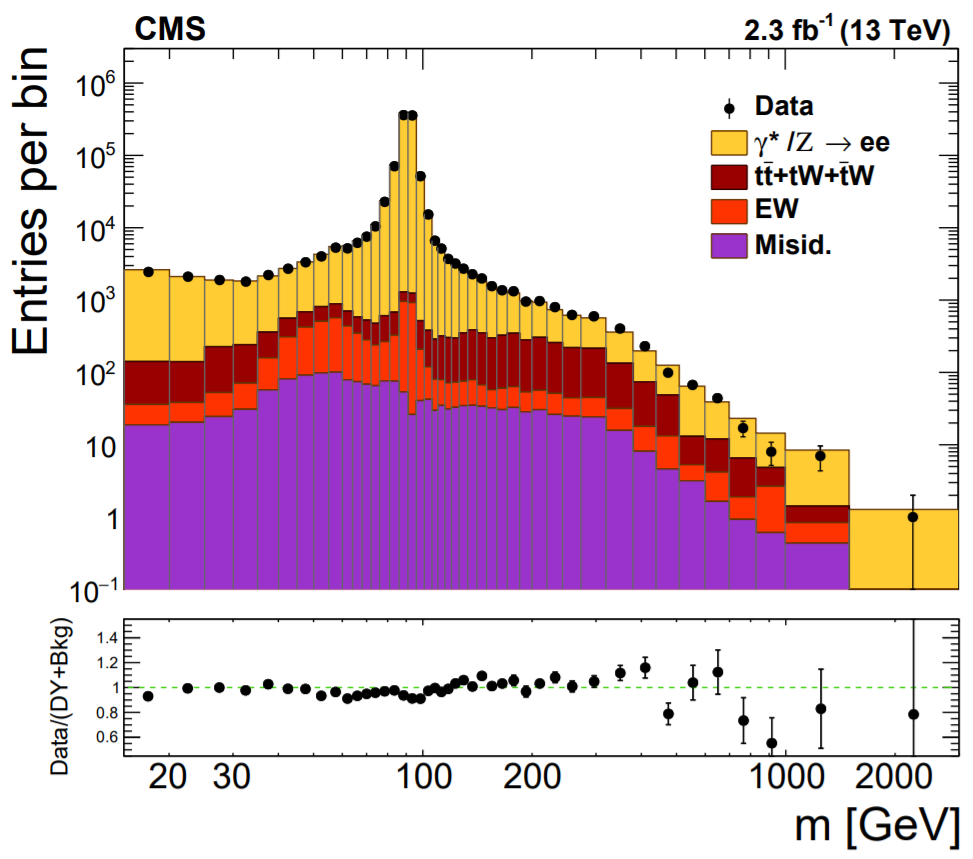
\includegraphics[width=.4\linewidth]{Figure1.png}
	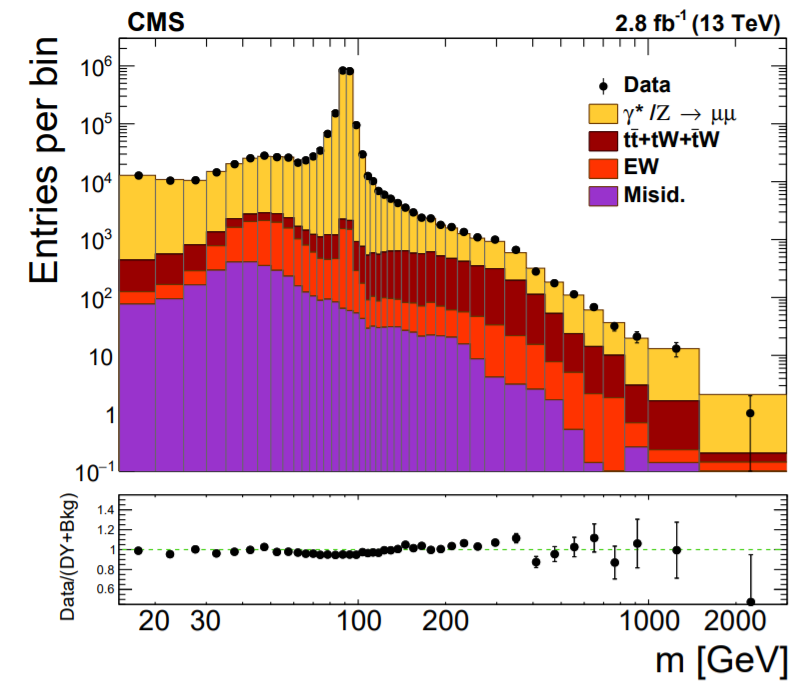
\includegraphics[width=.4\linewidth]{Figure2.png}
\vspace{-0.2cm}
\caption{Dielectron (left) and dimuon (right) invariant mass distributions measured using 2015 CERN CMS data \cite{DY13}.
      Black dots denote event yields measured with the CMS detector.    
      Yellow bars denote simulated Drell-Yan process.
      ``EW'' marks prompt lepton backgrounds.
      ``Misid.'' denotes fake lepton backgrounds, estimated using the ``fake rate'' method.}
\end{figure}

\vspace{-0.5cm}
\begin{thebibliography}{References}
\bibitem{DY}S.\ D.\ Drell, T.\ M.\ Yan, Massive Lepton Pair Production in Hadron-Hadron Collisions at High-Energies,
Phys.\ Rev.\ Lett.\ \textbf{25}, 316 (1970).

\bibitem{DY13}CMS Collaboration, Measurement of the differential Drell-Yan cross section in proton-proton collisions
at $\sqrt{s}=13$ TeV, JHEP \textbf{12} 059 (2019).

\bibitem{Higgs}ATLAS Collaboration. A search for the dimuon decay of the Standard Model Higgs boson with the ATLAS detector.
Phys.\ Lett.\ B \textbf{812}, 135980 (2021).

\bibitem{Zprime}CMS Collaboration. Search for high-mass resonances in dilepton final states in proton-proton collisions
at $\sqrt{s}=13$ TeV. JHEP \textbf{06} 120 (2018).

\bibitem{SUSY}CMS Collaboration. Search for top squark pair production using dilepton final states in pp collision data
collected at $\sqrt{s}=13$ TeV. Eur.\ Phys.\ J.\ C \textbf{81} 3 (2021).
\end{thebibliography}

\end{document}
